\chapter{Aporte práctico}
\label{cap:aporte_practico}
En el capítulo 3 se presentaron algunas técnicas y herramientas que sirven para el aprendizaje colaborativo; No obstante, para objetivos de esta tesis, se requiere una herramienta que integre ciertas características de las que ya poseen las mencionadas en el capítulo anterior.  \autoref{tab:herramientasAC}.\\

El sistema que se pretende desarrollar estará basado en el proceso para la elaboración de sesiones de clase usando la técnica de Jigsaw en la cual, tanto los grupos expertos y grupos jigsaw serán generados aleatoriamente por el sistema, garantizando así una mayor interacción entre los estudiantes, especialmente entre aquellos que se conocen por primera vez. \autoref{tab:tecnicasAC}.\\

El sistema a desarrollar también tendrá la particularidad de que permitirá a los estudiantes trabajar de forma colaborativa en la elaboración de archivos de código fuente, los cuales serán producto de las respuestas que dichos estudiantes darán a los problemas que les plantee el profesor durante la sesión de clase jigsaw. Por ende, para lograr este objetivo y tener dicha funcionalidad en el sistema, se usará los frameworks y APIs descritas en el capítulo anterior.  \autoref{tab:frameworks}.\\

Finalmente, para el desarrollo del sistema web, al cual de ahora en adelante llamaremos \textbf{Sistema Jigsaw Coding}, se va a considerar como proceso de desarrollo a las mejores prácticas de RUP para garantizar un producto software de calidad.

\section{Metodología de desarrollo}
Como ya se mencionó anteriormente, el Sistema Jigsaw Coding será elaborado usando las mejores prácticas de RUP, el mismo que a continuación se describe brevemente:\\

EL Proceso Unificado Rational(RUP) es un proceso de ingeniería de software que provee un enfoque para la asignación de tareas y responsabilidades durante el desarrollo de un software. Este tiene como objetivo asegurar la producción de un producto software de alta calidad que satisfaga los requerimientos de los usuarios finales dentro de un tiempo y presupuesto establecido \cite{rup_ibm_2014}. RUP, divide el proceso de desarrollo en fases y agrupa las diversas tareas y actividades en disciplinas, permitiendo organizar eficientemente cada uno de los artefactos que serán producto del desarrollo del sistema. \autoref{fig:rup}\\

\begin{figure}[!h]
  \centering
  % Requires \usepackage{graphicx}
  \fbox{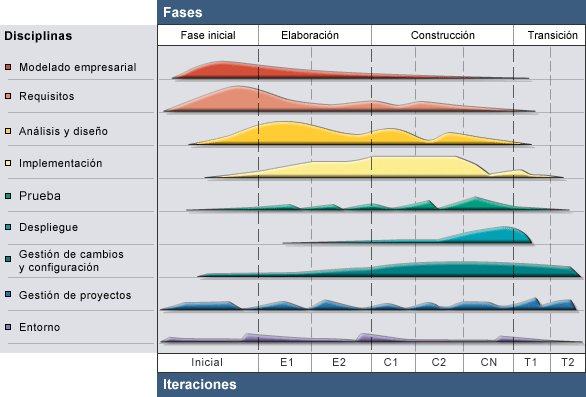
\includegraphics[scale=0.7]{figuras/rup.jpg}}\\
  \caption[RUP]{Proceso de desarrollo de software - RUP \protect\cite{rup_small}}\label{fig:rup}
\end{figure}

Así mismo, RUP también es una guía para usar de manera efectiva el Lenguaje Unificado de Modelado (UML) que no es más que un lenguaje estándar que permite comunicar claramente los requerimientos, arquitecturas y diseños \cite{rup_ibm_2014}.\\

Para el desarrollo del Sistema Jigsaw Coding, se establecerán iteraciones semanales en las cuales se irá desarrollando cada una de las fases en las que RUP divide el ciclo de desarrollo de software: Inicio, Elaboración, Construcción y Transición. Los artefactos que serán entregados durante el proceso de desarrollo del sistema propuesto en esta tesis se mencionan en la  \autoref{tab:artefactos_rup}. Además, dichos artefactos se encuentran agrupados según la disciplina a la que pertenecen.

\begin{longtable}{|L{6cm}|L{7cm}|}
\caption{Artefactos del proceso de desarrollo del Sistema Jigsaw Coding}
\label{tab:artefactos_rup}\\
	\toprule[0.8mm]
    DISCIPLINA RUP & ARTEFACTO \\
    \midrule
    \multirow{2}{*}{Requisitos} & $\bullet$ Modelo de caso de uso\\
    \hhline{~~} & $\bullet$ Especificaciones de casos de uso\\
    \hhline{~~} & $\bullet$ Especificaciones suplementarias\\
    \midrule
    \multirow{5}{*}{Análisis y diseño} & $\bullet$ Diagrama de clases\\
    \hhline{~~} & $\bullet$ Modelo de datos\\
    \hhline{~~} & $\bullet$ Prototipo de interfaz de usuario\\
    \hhline{~~} & $\bullet$ Documento de arquitectura de software\\
    \midrule
    \multirow{2}{*}{Implementación} & $\bullet$ Código fuente\\
    \hhline{~~} & $\bullet$ Sistema web desplegado\\
    \midrule
    \multirow{2}{*}{Prueba} & $\bullet$ Casos de prueba\\
    \hhline{~~} & $\bullet$ Resultados de prueba\\
    \bottomrule[0.8mm]
\end{longtable}

\clearpage
%Para el desarrollo del sistema web, se seguirá el siguiente cronograma, el mismo que se está orientado a seguir las actividades y tareas que plantea RUP. Se indica también las fechas en las cuales se estará aplicando el sistema al caso de estudio.
%
%\begin{figure}[!h]
%  \centering
%  % Requires \usepackage{graphicx}
%  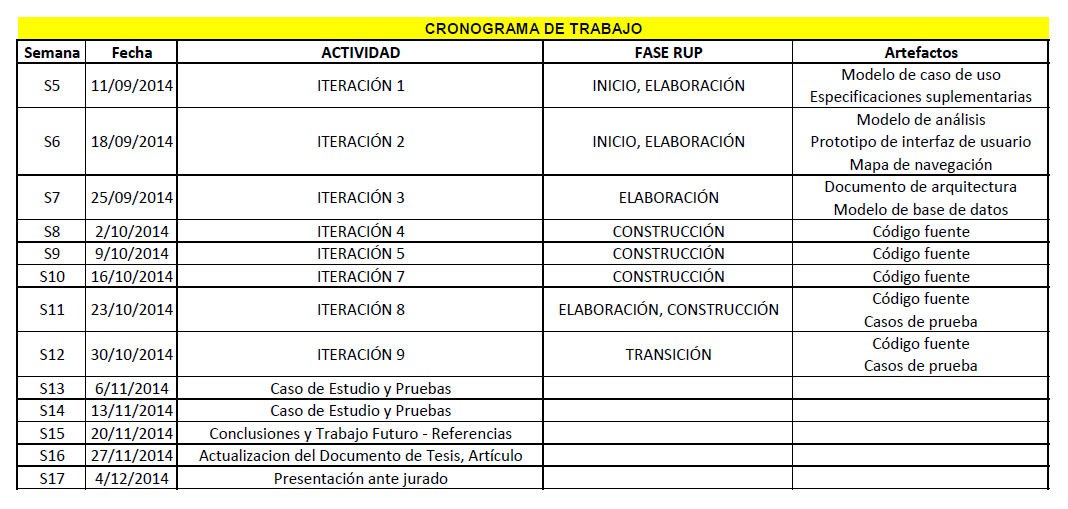
\includegraphics[scale=0.5]{figuras/cronograma.png}\\
%  \caption[CRONOGRAMA]{Cronograma de trabajo}\label{fig:cronograma}
%\end{figure}

%\begin{longtable}{|L{2.5cm}|L{2cm}|L{5cm}|L{5cm}|}
%\caption{CRONOGRAMA}
%\label{tab:cronograma}\\
%    \hline
%    ITERACIÓN & FECHA & FASE RUP & ARTEFACTO \\
%    \hline
%    1 &	11-09-2014	&	INICIO, ELABORACIÓN	& Modelo de caso de uso, Especificaciones suplementarias\\
%
%    \hline
%\end{longtable}

\section{Desarrollo del Sistema Jigsaw Coding}
En esta sección se presenta una descripción a alto nivel sobre los artefactos elaborados durante el proceso de desarrollo del sistema.

\subsection{Modelo de casos de uso}
El modelo de casos de uso permite mostrar de manera general las funcionalidades del sistema. Inicialmente, se indica el catálogo de actores que interactúan con el sistema y luego se presenta la descripción de lo casos de uso más resaltantes. La especificación de todos los casos de uso se encuentra en el \autoref{apendice.A}\\

Los casos de uso son una forma de especificación de requisitos funcionales. Un caso de uso es la descripción de una secuencia de interacciones entre el sistema y un o más actores.\\

\subsubsection{Catálogo de actores}
En el la \autoref{fig:cap4_actores} se puede ver los actores que participan en el Sistema Jigsaw Coding y en la \autoref{tab:cap4_actores} se encuentra una breve descripción de cada uno de ellos.
\begin{figure}
	\centering
	% Requires \usepackage{graphicx}
	\fbox{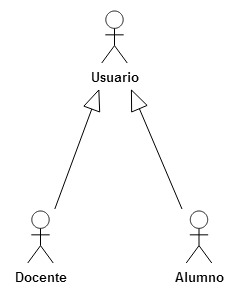
\includegraphics[scale=0.6]{figuras/casosdeuso/actores.jpg}}\\
	\caption[Diagrama de actores]{Diagrama de actores}
	\label{fig:cap4_actores}
\end{figure}
\clearpage
\begin{longtable}{L{3cm}L{7cm}}
	\caption{Actores}
	\label{tab:cap4_actores}\\
	\toprule[0.8mm]
	ACTOR & DESCRIPCIÓN \\
	\midrule[0.6mm]
	Usuario & Persona que usará el sistema web de tiempo real para el aprendizaje colaborativo.\\
	\midrule
	Docente & Es la persona responsable de crear y dirigir las sesiones de clase que serán aplicadas a los alumnos. Además, el docente es el responsable de las evaluaciones que rendirán los alumnos una vez terminada cada sesión de clase.\\
	\midrule
	Alumno & Es la persona que será instruida en temas de algoritmos y programación a través de cada sesión diseñada por el docente.\\
	\bottomrule[0.8mm]
\end{longtable}

\subsubsection{Casos de uso}
En la tabla siguiente se presenta la descripción breve de los casos de uso obtenidos para el Sistema Jigsaw Coding, estos son especificados de una manera más detallada en el \autoref{apendice.A}
\begin{longtable}{L{4cm}L{9cm}}
	\caption{Casos de uso}
	\label{tab:cap4_casosdeuso}\\
	\toprule[0.8mm]
	CASO DE USO & DESCRIPCIÓN \\
	\midrule[0.6mm]
	Registrar alumno & Este caso de uso define los pasos que el usuario con perfil docente debe seguir para poder registrar un alumno en el sistema.\\
	\midrule
	Crear Problema & El caso de uso crear problema detalla la interacción entre el sistema y el usuario docente cada vez que éste necesite crear un problema o ejercicio en el sistema.\\
	\midrule
	Crear sesión jigsaw & Este caso de uso describe la secuencia de pasos que se debe seguir para poder crear una sesión de clase basada en la técnica de aprendizaje colaborativo jigsaw.\\
	\midrule
	Asignar alumnos a sesión jigsaw & Las sesiones jigsaw necesitan tener alumnos y ese es el objetivo que tine este caso de uso.\\
	\midrule
	Generar grupos & Mediante este caso de uso, el Sistema Jigsaw Coding realiza la creación de grupos expertos y grupos jigsaw y a cada uno de ellos les asigna alumnos de forma aleatoria.\\
	\midrule
	Asignar problemas a grupos expertos & En este caso de uso se describe cómo el usuario docente puede asignar un problema a cada grupo experto generado por el sistema para una determinada sesión jigsaw.\\
	\midrule
	Crear examen & El caso de uso detalla la manera en la que el usuario docente puede crear un examen, el mismo que será usado para la fase de evaluación de la sesión jigsaw.\\
	\midrule
	Definir horario de reunión de expertos & Este caso de uso sirve para establecer la fecha y hora de inicio de la reunión de expertos así como su respectiva duración.\\
	\midrule
	Definir horario de reunión jigsaw & Este caso de uso sirve para establecer la fecha y hora de inicio de la reunión jigsaw así como su respectiva duración.\\
	\midrule
	Definir horario de examen & Este caso de uso sirve para establecer el intervalo de tiempo en el cual se puede acceder a examen así como también su respectiva duración.\\
	\midrule
	Unirse a reunión de expertos & Este caso de uso le sirve al usuario alumno para poder ingresar a la reunión de expertos y desarrollar el problema asignado junto con los demás integrantes del grupo.\\
	\midrule
	Unirse a reunión jigsaw & Este caso de uso le sirve al usuario alumno para poder ingresar a la reunión jigsaw y desarrollar los respectivos problemas junto con los demás integrantes del grupo. \\
	\midrule
	Resolver problema & El caso de uso describe la interacción entre el usuario alumno y el sistema cada vez que se requiere resolver un problema asignado por el usuario docente.\\
	\midrule
	Rendir examen & El caso de uso le permite al usuario alumno acceder al examen y visualizar cada una de las preguntas que debe resolver.\\
	\midrule
	Consultar al grupo & Este caso de uso describe la manera en la que un usuario alumno puede consultar con los demás integrantes de su grupo experto o grupo jigsaw.\\
	\bottomrule[0.8mm]
\end{longtable}

\subsection{Arquitectura del Sistema}
En esta sección se provee una vista general de la arquitectura para el Sistema Jigsaw Coding, la misma que permite tener una visión sobre la estructura del sistema, funcionalidades y demás aspectos técnicos que el sistema requiere.\\

La meta principal del Sistema Jigsaw Coding es que opere sobre una plataforma web y para esto es necesario utilizar herramientas y tecnologías que permitan desarrollar sistemas web. Además debe tenerse en cuenta ciertos frameworks que ayuden en la elaboración de la parte colaborativa del sistema.

\subsubsection{PlayFramework 2.2.4}
Play es framework open source de Java y Scala que integra componentes y APIs necesarios para el desarrollo moderno de aplicaciones web. Play sigue el patrón de arquitectura Modelo - Vista - Controlador y uno de sus objetivos es optimizar la productividad del desarrollador a través del uso de configuraciones estandarizadas, recompilación automática del código fuente y la visualización de errores directamente en el navegador.

\subsubsection{Persistencia}
La persistencia se logrará utilizando una base de datos relacional y el mapeo de entidades a tablas estará a cargo del ORM Ebean que por defecto viene incluído en el framework Play.

\subsubsection{Seguridad}
La seguridad del sistema está basada en perfiles. La aplicación contendrá los siguientes puntos:

\begin{itemize}
	\item Autenticación: Cada usuario deberá identificarse con su email y password para poder acceder al sistema.
	\item Autorización: El sistema cuenta con dos perfiles(Docente y Alumno) y dependiendo de ello, el usuario podrá ingresar a diferentes partes del sistema.
	\end{itemize}

\subsubsection{Vista lógica}
\begin{figure}[!h]
\centering
% Requires \usepackage{graphicx}
\fbox{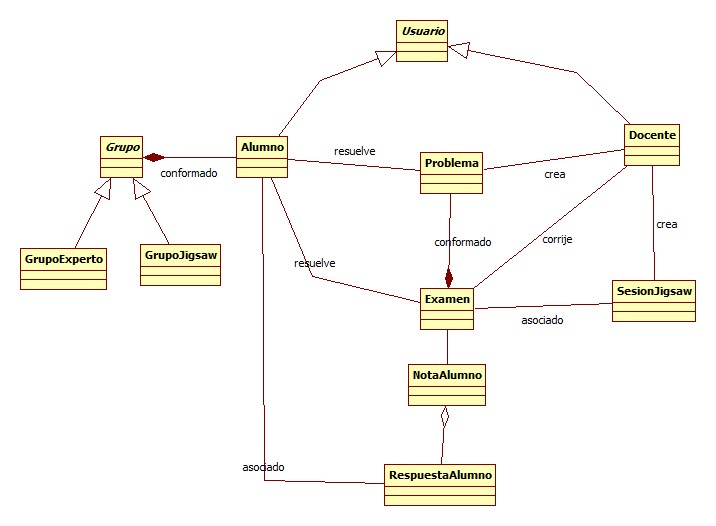
\includegraphics[scale=0.5]{figuras/sad/diagrama_de_clases.jpg}}\\
\caption{Diagrama de Clases}\label{fig:c4_diagrama_de_clases}
\end{figure}

El Sistema Jigsaw Coding permite el acceso a Usuario lo cuales pueden ser de dos tipos: Docente o Alumno. El docente puede crear problemas y además es el encargado de crear las sesiones jigsaw. El docente también es quien crea los examenes, los cuales están conformados por un conjunto de problemas y cada examen es resuelto por los alumnos, quienes para tal objetivo, deben resolver los problemas que componen cada examen. Por otro lado, los alumnos también resuelven problemas cada vez que se encuentran dentro de un grupo de expertos o un grupo jigsaw. Naturalmente, los examenes son evaluados por el docente y éste les asigna una nota a cada una de las respuestas que los alumnos envía al terminar su examen.

\subsubsection{Vista de Desarrollo}
La vista de desarrollo muestra el sistema desde la perspectiva del programador y se ocupa de la gestión del software a implementar. Esto es, en esta vista se describe cómo estará dividido el sistema Jigsaw Coding en paquetes y las dependencias que hay entre ellos.
\begin{figure}[!h]
	\centering
	% Requires \usepackage{graphicx}
	\fbox{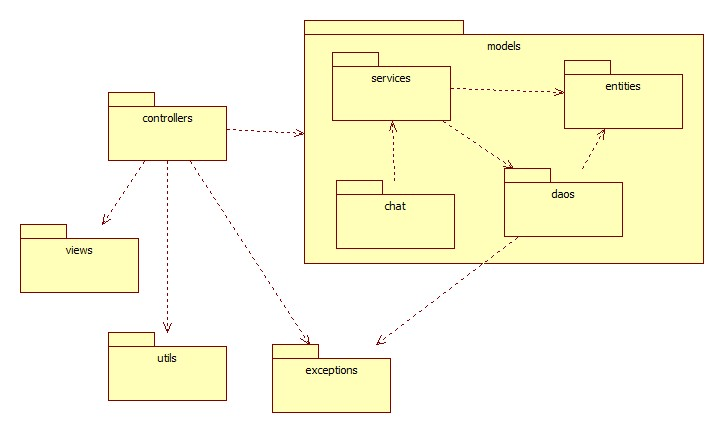
\includegraphics[scale=0.5]{figuras/sad/diagrama_de_paquetes.jpg}}\\
	\caption{Diagrama de Paquetes}\label{fig:c4_diagrama_de_paquetes}
\end{figure}
\begin{itemize}
	\item \textbf{controllers}\\Este paquete contiene todas las clases Controladores que sirven para gestionar el ruteo de páginas del sistema.
	\item \textbf{models}\\En este paquete se encuentran las clases de Servicios, Entidades y Acceso a Datos que son requeridas para el sistema.
	\item \textbf{views}\\Este paquete contiene todas las plantillas (\emph{*.scala.html}) que permitirán renderizar las páginas web del sistema.
\end{itemize}

Para un mayor detalle de la arquitectura del sistema, revisar el \autoref{apendice.C}

\section{Uso del Sistema Jigsaw Coding} 
El Sistema Jigsaw Coding es un aplicativo web que permite crear sesiones de clase basadas en la técnica de aprendizaje colaborativo de rompecabezas o también llamada técnica jigsaw. Estas sesiones de clase están orientadas a la resolución de ejercicios y problemas relacionados con temas de algorítmica y programación en lenguajes Java, C++ y Python.\\

El sistema posee dos perfiles de usuario: Docente y Alumno. El primero permite al usuario crear ejercicios y problemas de algoritmos y programación. Dentro del perfil docente, el usuario tiene la capacidad para crear a los usuarios alumnos que participarán en la sesión de clase jigsaw para luego asignarlos a las sesiones jigsaw para que el sistema genere los grupos expertos y grupos jigsaw. Posteriormente a ello, el usuario con perfil docente podrá asignar a cada grupo experto un problema o ejercicio a resolver, y luego asignar la fecha y duración para cada fase de la dinámica jigsaw (Reunión de Expertos, Reunión Jigsaw y Evaluación). Para la fase de evaluación, el sistema permite al usuario crear diversos examenes con problemas y ejercicios a los cuales se les asigna un puntaje; luego, cada examen se asigna a una determinada sesión jigsaw. Finalmente, el usuario docente podrá calificar la solución que cada uno de los participantes de la sesión jigsaw elabore para un determinado examen.\\

En el perfil Alumno, el usuario puede participar de las reuniones de expertos y reunions jigsaw, en las cuales se deberá resolver los problemas asignados a cada grupo experto o jigsaw. Esta soluciones serán construidas de forma colaborativa entre todos los miembros de cada grupo. El sistema brinda al usuario un chat para poder comunicarse con los demás integrantes de su grupo experto o jigsaw. Es importante resaltar también, que durante la resolución de cada problema el usuario puede ir ejecutando el código fuente y ver los resultados de dicha ejecución. Cuando el usuario se encuentre en la fase de evaluación, éste podrá resolver su examen de forma individual y dentro del tiempo establecido por el docente.\\

\subsection{Login} 
Para acceder al Sistema Jigsaw Coding, el usuario debe estar su \textbf{email} y su \textbf{password} en el formulario que se muestra en la \autoref{fig:sjc_login}.

\begin{figure}[h!]
	\centering
	\caption[SJC Login]{Sistema Jigsaw Coding - Login}
	\label{fig:sjc_login}
	\fbox{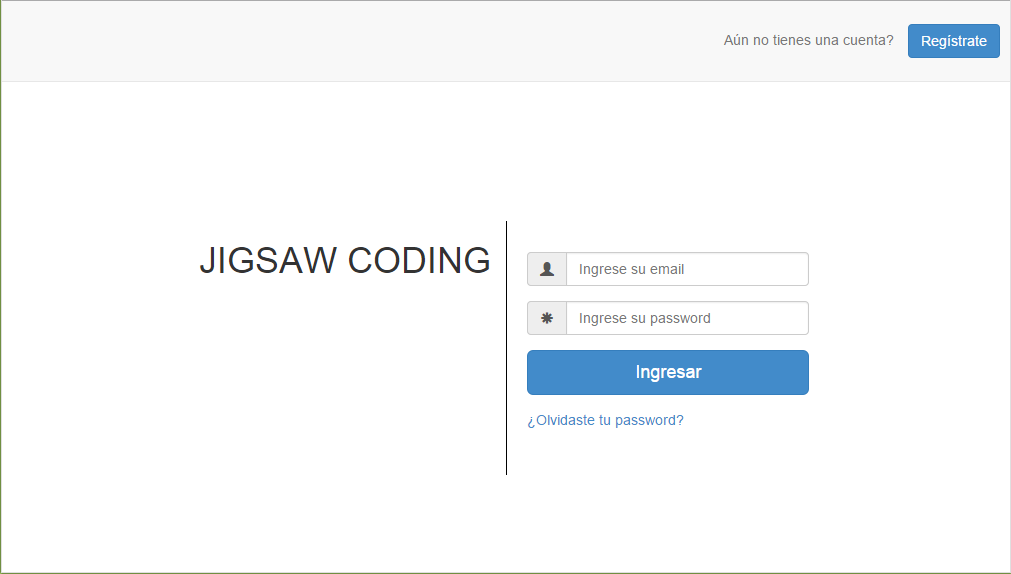
\includegraphics[scale=0.4]{figuras/usodelsistema/login}}	
\end{figure}

Si el usuario no está registrado en el sistema, debe ingresar a la opción \textbf{Regístrate} y completar los datos solicitados por el sistema. \autoref{fig:login_registrate}. Luego de este paso, el usuario tendrá acceso al sistema a través de un perfil Docente.\\

\begin{figure}[h!]
	\centering
	\caption[SJC Registrate]{Sistema Jigsaw Coding - Regístrate}
	\label{fig:login_registrate}
	\fbox{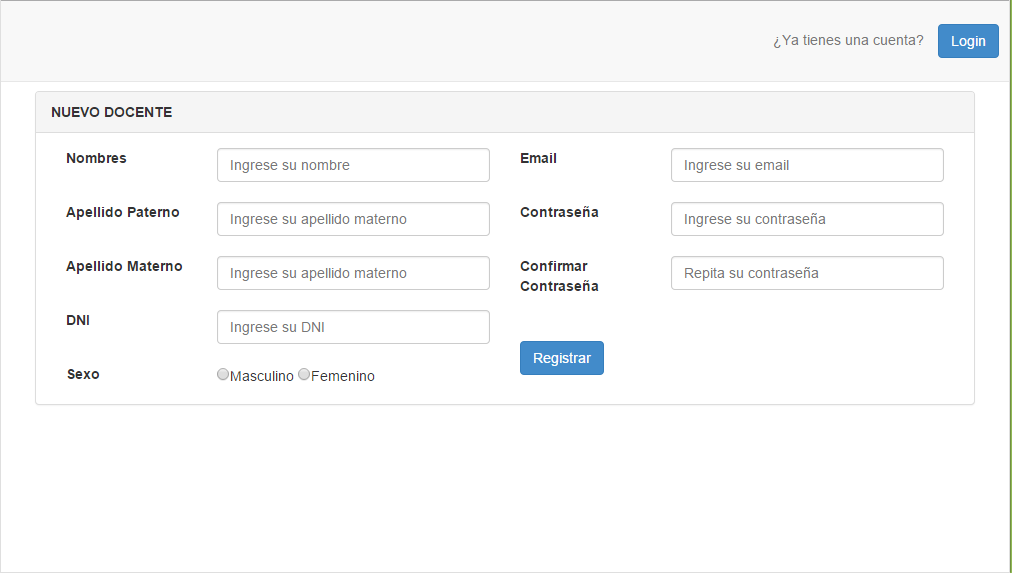
\includegraphics[scale=0.5]{figuras/usodelsistema/login_registrate}}	
\end{figure}

Si el acceso al sistema se dió exitosamente, entonces el usuario podrá visualizar la página de inicio con todas las opciones permitidas para el perfil docente. \autoref{fig:inicio}.

\begin{figure}[h!]
\centering
\caption[SJC Inicio]{Sistema Jigsaw Coding - Bienvenido}
\label{fig:inicio}
\fbox{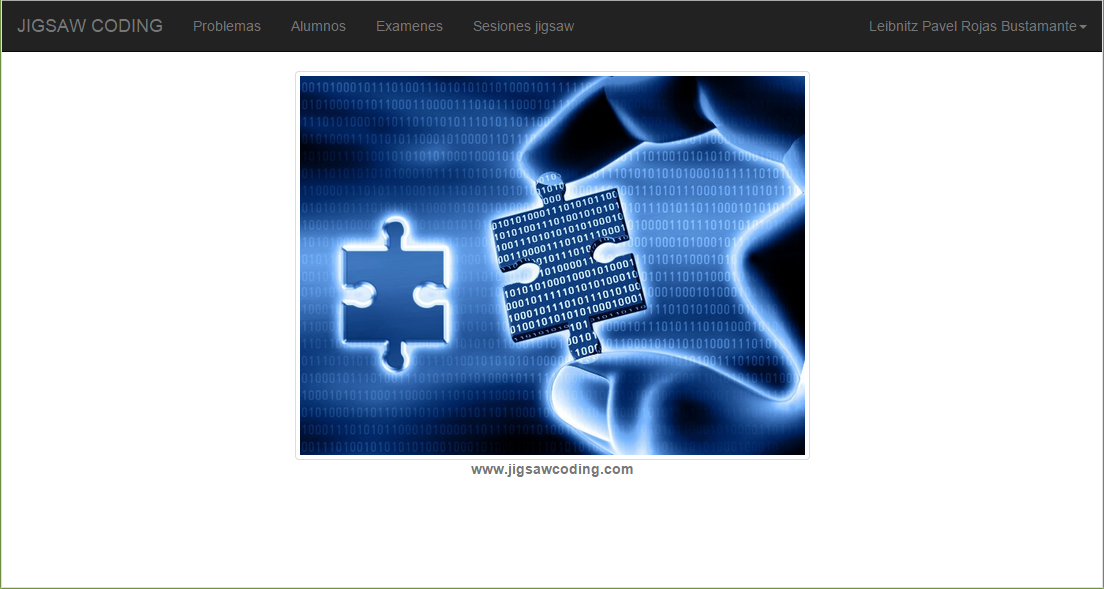
\includegraphics[scale=0.5]{figuras/usodelsistema/docente/inicio}}
\end{figure}
%\clearpage

\subsection{Problemas}
Al acceder al módulo problemas, el usuario visualizará el listado de problemas que ha creado hasta el momento y en dicho listado, se mostrará el título y enunciado de cada problema. Además se podrá filtrar los problemas según el título o enunciado. \autoref{fig:problemas_inicio}.

\begin{figure}[h!]
\centering
\caption[SJC Problemas]{Sistema Jigsaw Coding - Inicio del módulo Problemas}
\label{fig:problemas_inicio}
\fbox{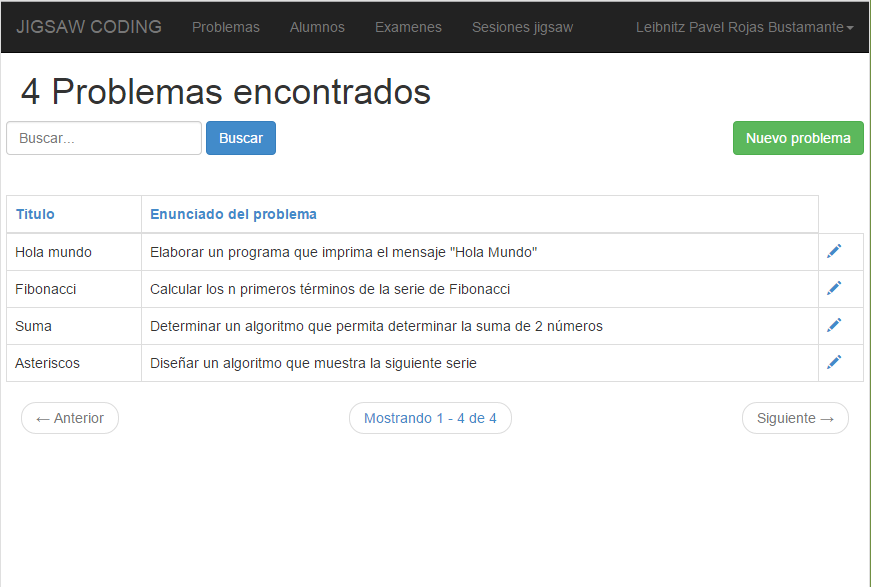
\includegraphics[scale=0.5]{figuras/usodelsistema/docente/problemas_inicio}}
\end{figure}

\subsubsection{Crear problema}

Para crear un nuevo problema se debe acceder a menú Problemas y luego presionar el botón \textbf{Nuevo problema}. \autoref{fig:problemas_nuevo}. Luego, se debe ingresar el título y enunciado del problema y presionar el botón \textbf{Guardar}.

\begin{figure}[h!]
\centering
\caption[SJC Nuevo problema]{Sistema Jigsaw Coding - Nuevo problema}
\label{fig:problemas_nuevo}
\fbox{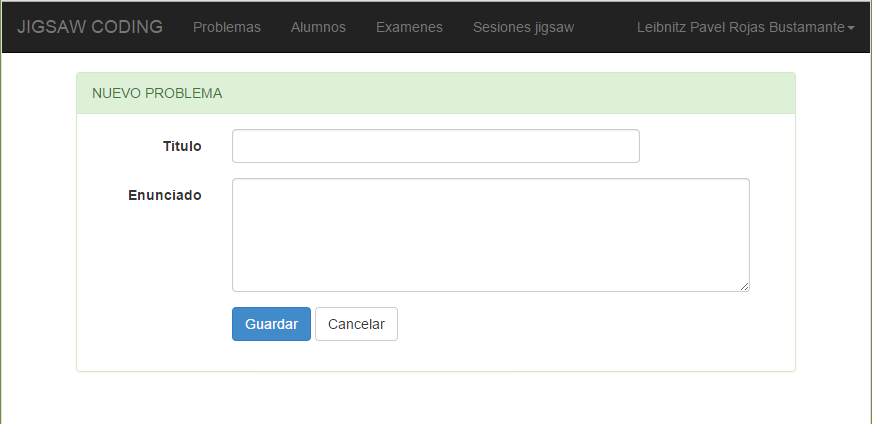
\includegraphics[scale=0.5]{figuras/usodelsistema/docente/problemas_nuevo}}
\end{figure}

\subsubsection{Editar problema}
En la página principal del módulo Problemas se puede ver cada problema creado y para cada uno, existe un botón que permite editar dicho problema. Con esta opción se puede modificar el título o enunciado del problema y también se puede eliminar dicho problema del sistema. Ver figura \autoref{fig:problemas_editar}.

\begin{figure}[h!]
\centering
\caption[SJC Editar problema]{Sistema Jigsaw Coding - Editar problema}
\label{fig:problemas_editar}
\fbox{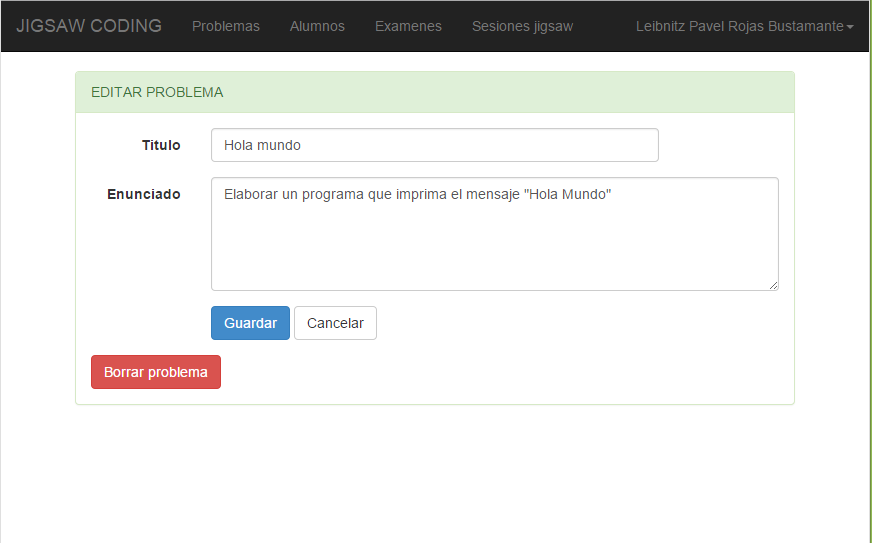
\includegraphics[scale=0.5]{figuras/usodelsistema/docente/problemas_editar}}
\end{figure}

\subsection{Alumnos}
Al acceder al módulo alumnos, el usuario visualizará el listado de alumnos registrados hasta el momento y en dicho listado, se mostrará los apellidos, nombres y dni de cada alumno. Además se podrá filtrar dichos alumnos con opción Buscar. \autoref{fig:alumnos_inicio}.

\begin{figure}[h!]
	\centering
	\caption[SJC Alumnos]{Sistema Jigsaw Coding - Inicio del módulo Alumnos}
	\label{fig:alumnos_inicio}
	\fbox{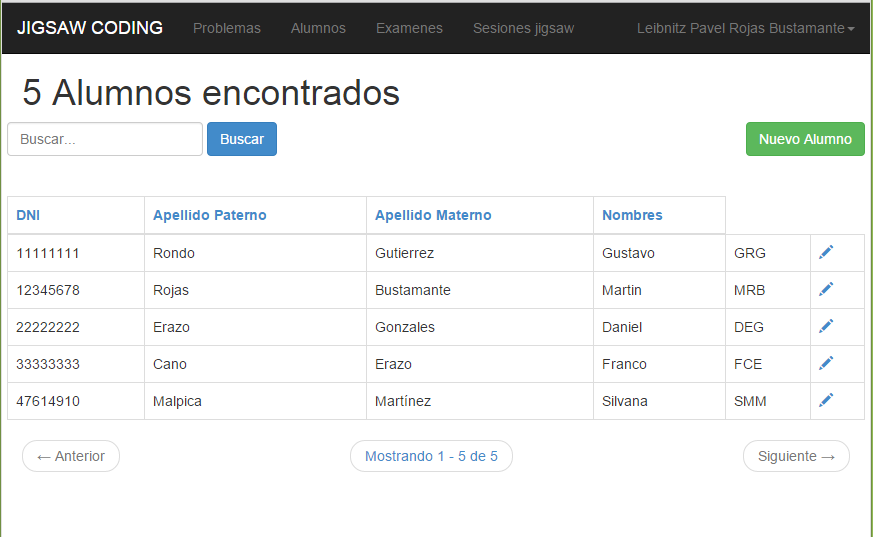
\includegraphics[scale=0.5]{figuras/usodelsistema/docente/alumnos_inicio}}
\end{figure}

\subsubsection{Registrar alumno}

Para registrar un nuevo alumno se debe acceder a menú Alumnos y luego presionar el botón \textbf{Nuevo Alumno}. \autoref{fig:alumnos_nuevo}. Luego, se debe completar los campos solicitados por el sistema y presionar el botón \textbf{Registrar}.

\begin{figure}[h!]
	\centering
	\caption[SJC Nuevo alumno]{Sistema Jigsaw Coding - Nuevo Alumno}
	\label{fig:alumnos_nuevo}
	\fbox{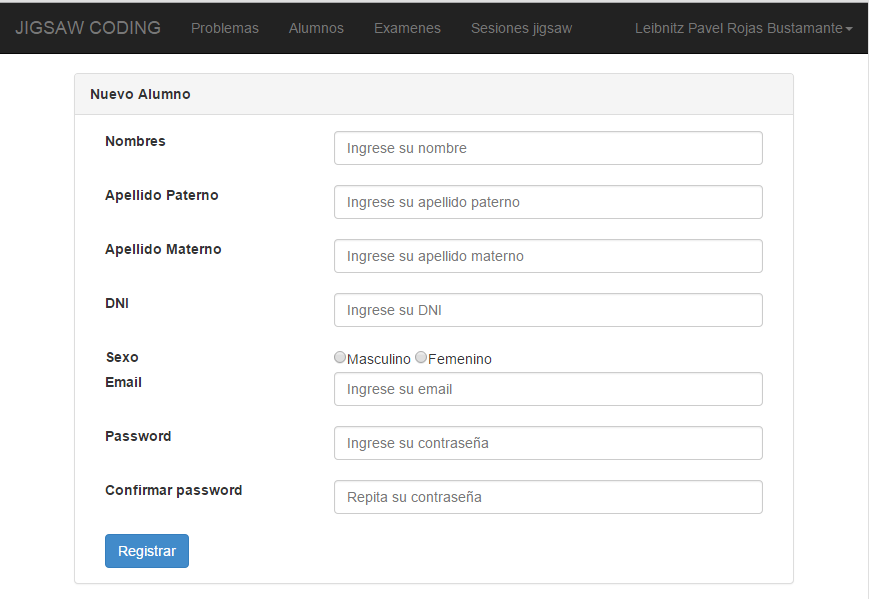
\includegraphics[scale=0.5]{figuras/usodelsistema/docente/alumnos_nuevo}}
\end{figure}

\subsection{Examenes}
Al acceder al módulo examenes, el usuario visualizará el listado de examenes registrados hasta el momento y en dicho listado, se mostrará el título del examen y los nombres de los problemas que forman parte del examen. Además se podrá filtrar dichos examenes con opción Buscar. \autoref{fig:examenes_inicio}.

\begin{figure}[h!]
	\centering
	\caption[SJC Examenes]{Sistema Jigsaw Coding - Inicio del módulo Examenes}
	\label{fig:examenes_inicio}
	\fbox{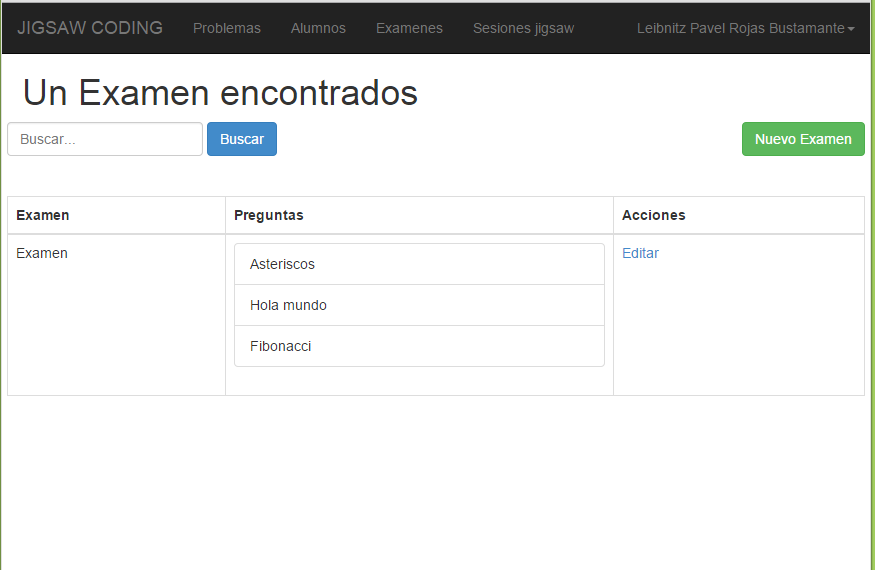
\includegraphics[scale=0.5]{figuras/usodelsistema/docente/examenes_inicio}}
\end{figure}
\subsubsection{Crear examen}

Para registrar un nuevo examen se debe acceder a menú Examenes y luego presionar el botón \textbf{Nuevo Examen} con lo cual el usuario podrá ver la interfaz para asignar los problemas al examen. \autoref{fig:examenes_nuevo}. \\

\begin{figure}[h!]
	\centering
	\caption[SJC Nuevo examen]{Sistema Jigsaw Coding - Nuevo Examen}
	\label{fig:examenes_nuevo}
	\fbox{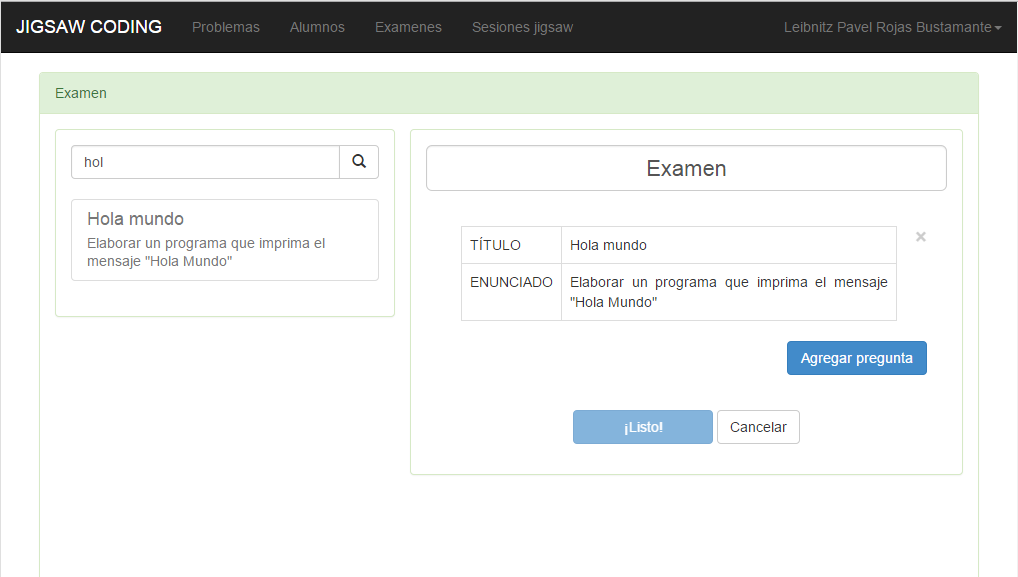
\includegraphics[scale=0.5]{figuras/usodelsistema/docente/examenes_nuevo}}
\end{figure}

La asignación de problemas al examen se realiza siguiendo los pasos descritos a continuación:

\begin{enumerate}
	\item En el campo \textbf{Buscar} escriba el nombre del problema que desea agregar.
	\item Haga click en el problema y automáticamente éste se mostrará en el panel del Examen.
	\item Presione el botón Agregar pregunta.
	\item Haga click en el problema para habilitar las opciones de asignar puntaje al problema y establezca la puntación para el problema. 
	\item Presione nuevamente el problema para guardar el puntaje.
	\item Agregue los problemas que sean necesarios hasta que el marcador de puntaje de examen sume un total de 20 puntos. Luego entonces presione el botón \textbf{Listo} para guardar el examen.
\end{enumerate}

\subsection{Sesiones Jigsaw}
Al acceder al módulo sesiones jigsaw, el usuario podrá ver el listado de sesiones jigsaw creadas hasta el momento y en dicho listado se encontrará la respectiva información sobre la reunión de expertos, reunión jigsaw y evaluación. \autoref{fig:sesionesjigsaw_inicio}.

\begin{figure}[h!]
\centering
\caption{Sistema Jigsaw Coding - Inicio del módulo sesiones jigsaw}
\label{fig:sesionesjigsaw_inicio}
\fbox{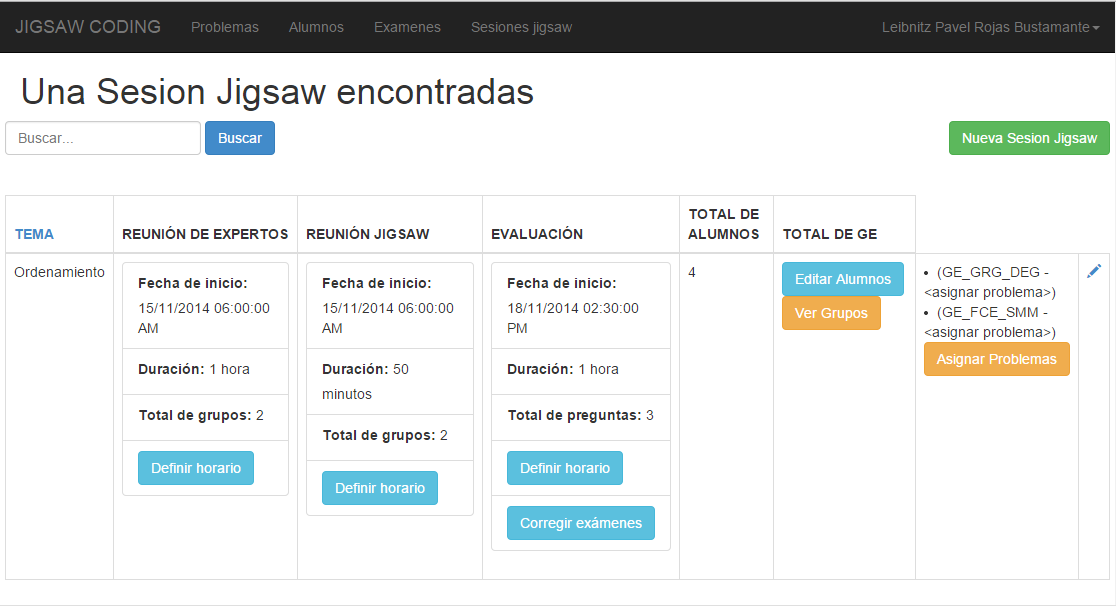
\includegraphics[scale=0.5]{figuras/usodelsistema/docente/sesionesjigsaw_inicio}}
\end{figure}
%\clearpage
\subsubsection{Crear sesión jigsaw}
A continuación se describen los pasos para crear una sesión jigsaw.
\begin{enumerate}
	\item Presione el botón \textbf{Nueva Sesión Jigsaw}.
	\item Indique el total de grupos expertos y el tema de la sesión jigsaw. \autoref{fig:sesionesjigsaw_nuevo_01}
	\begin{figure}[h!]
	\centering
	\caption[SJC Sesiones jigsaw]{Sistema Jigsaw Coding - Nueva sesión jigsaw}
	\label{fig:sesionesjigsaw_nuevo_01}
	\fbox{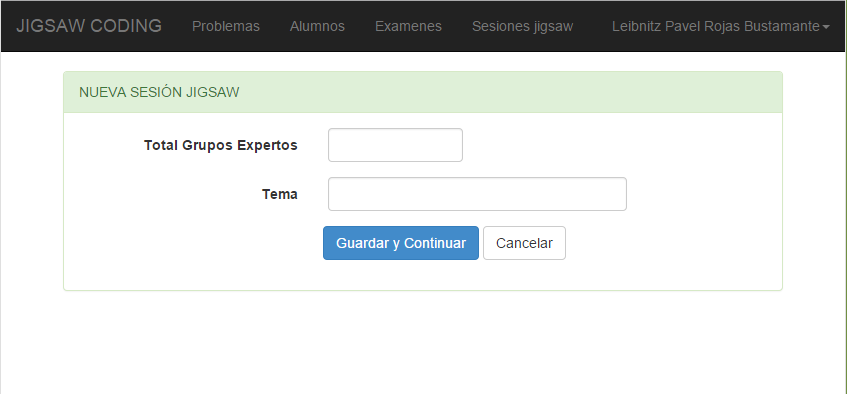
\includegraphics[scale=0.5]{figuras/usodelsistema/docente/sesionesjigsaw_nuevo_01}}
	\end{figure}
	\item En el listado de sesiones jigsaw aparecerá una nueva sesión.\autoref{fig:sesionesjigsaw_nuevo_02}
	\begin{figure}[h!]
	\centering
	\caption{Sistema Jigsaw Coding - Nueva sesión jigsaw}
	\label{fig:sesionesjigsaw_nuevo_02}
	\fbox{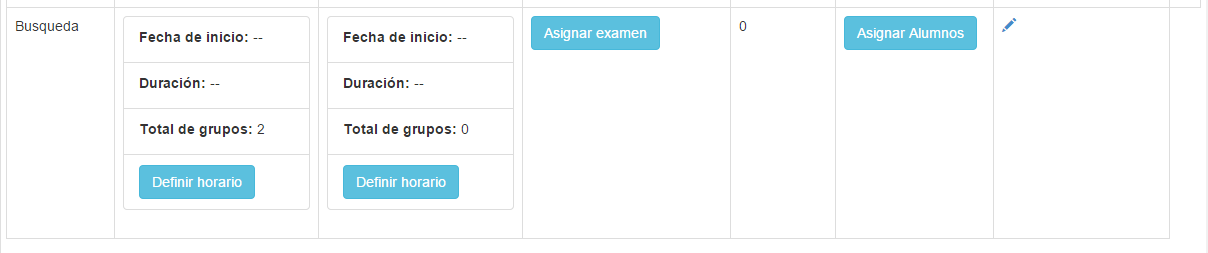
\includegraphics[scale=0.5]{figuras/usodelsistema/docente/sesionesjigsaw_nuevo_02}}
	\end{figure}
	\item Presione el botón agregar alumnos para definir qué alumnos formarán parte de la sesión jigsaw. Mueva los alumnos desde el panel de Alumnos Disponibles hacia el panel de la Sesión Jigsaw y presione el botón \textbf{Guardar}.  \autoref{fig:sesionesjigsaw_nuevo_03}
	\begin{figure}[h!]
	\centering
	\caption{Sistema Jigsaw Coding - Nueva sesión jigsaw}
	\label{fig:sesionesjigsaw_nuevo_03}
	\fbox{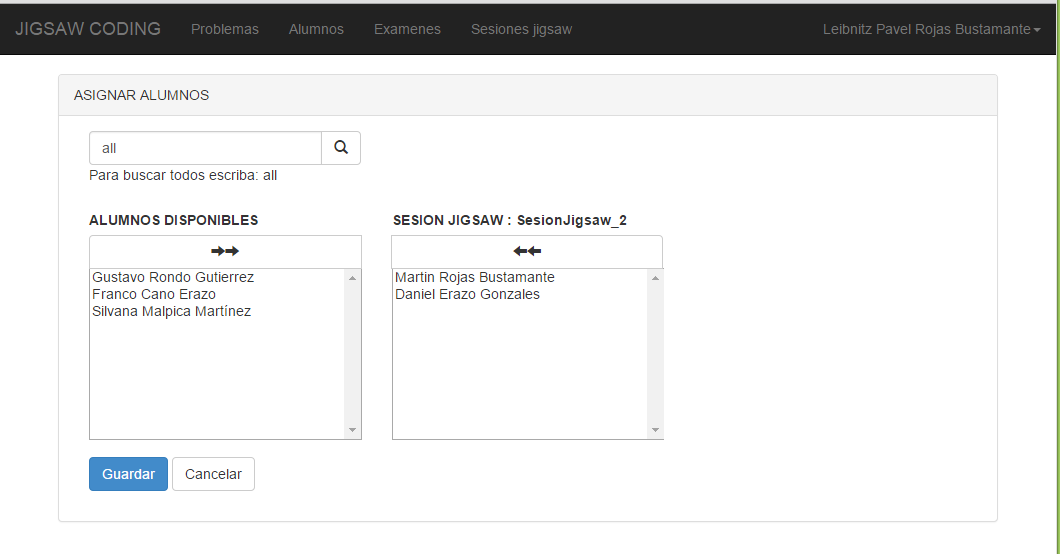
\includegraphics[scale=0.5]{figuras/usodelsistema/docente/sesionesjigsaw_nuevo_03}}
	\end{figure}
	\item Luego de agregar a los alumnos, se habilitará el botón Generar Grupos el cual deberá presionar para que el sistema genere de forma aleatoria los Grupos expertos y los grupos jigsaw. \autoref{fig:sesionesjigsaw_nuevo_04}
	\begin{figure}[h!]
		\centering
		\caption{Sistema Jigsaw Coding - Nueva sesión jigsaw}
		\label{fig:sesionesjigsaw_nuevo_04}
		\fbox{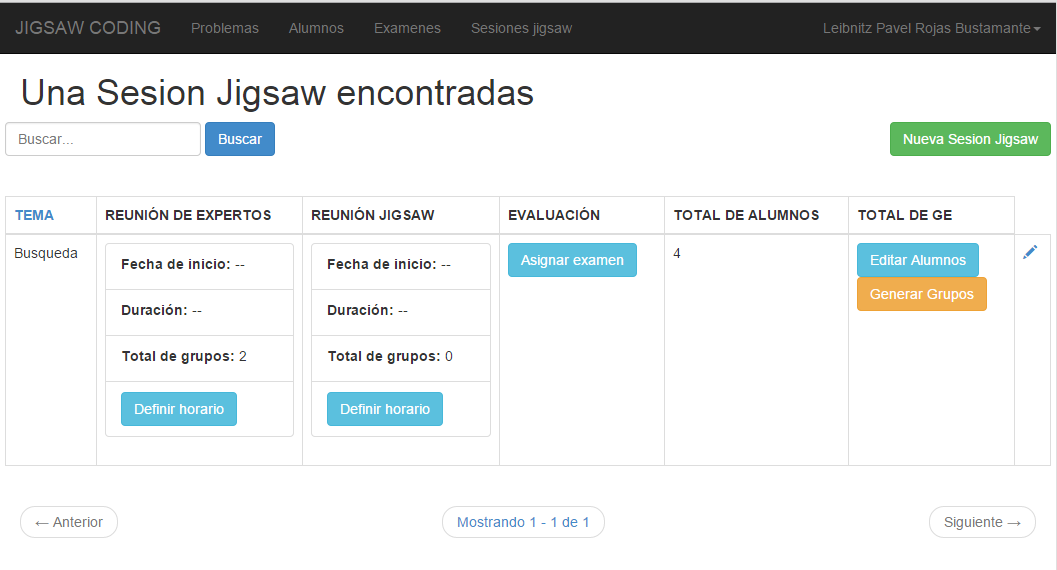
\includegraphics[scale=0.5]{figuras/usodelsistema/docente/sesionesjigsaw_nuevo_04}}
	\end{figure}
	\item Si la generación de grupos se realizó exitosamente, el sistema le mostrará los grupos sus respectivos integrantes. \autoref{fig:sesionesjigsaw_nuevo_05}
	\begin{figure}[h!]
		\centering
		\caption{Sistema Jigsaw Coding - Nueva sesión jigsaw}
		\label{fig:sesionesjigsaw_nuevo_05}
		\fbox{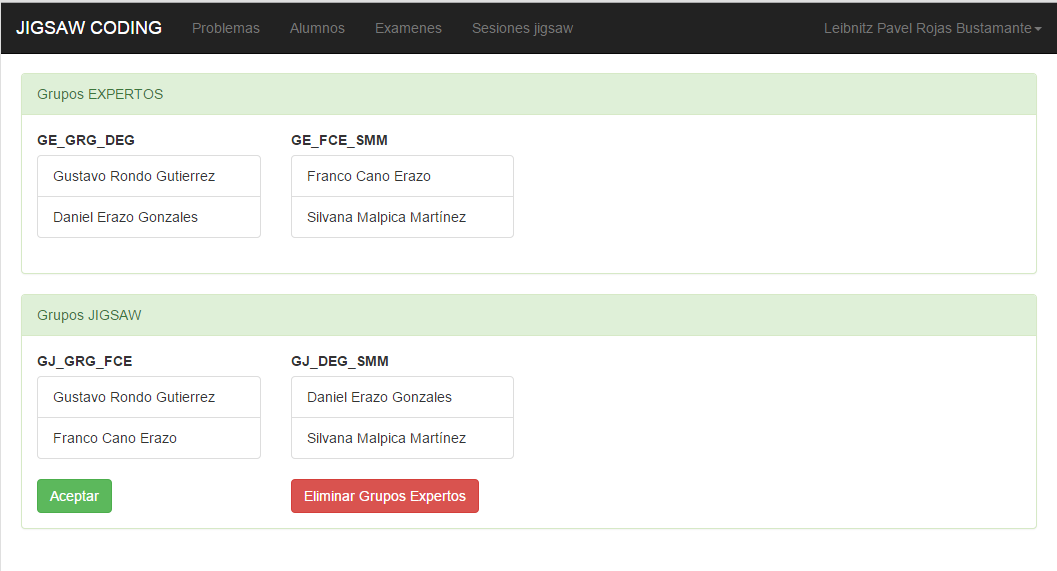
\includegraphics[scale=0.5]{figuras/usodelsistema/docente/sesionesjigsaw_nuevo_05}}
	\end{figure}
	\item Presione Aceptar para regresar al panel principal de las sesiones jigsaw. \autoref{fig:sesionesjigsaw_nuevo_06}
	\begin{figure}[h!]
		\centering
		\caption{Sistema Jigsaw Coding - Nueva sesión jigsaw}
		\label{fig:sesionesjigsaw_nuevo_06}
		\fbox{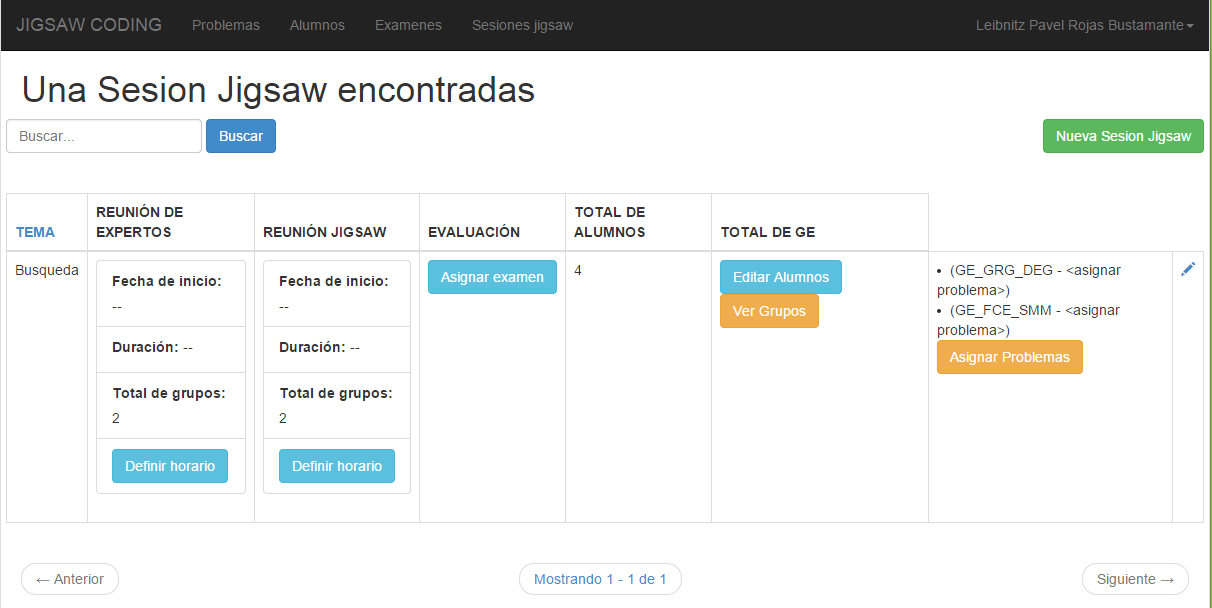
\includegraphics[scale=0.5]{figuras/usodelsistema/docente/sesionesjigsaw_nuevo_06}}
	\end{figure}
	\item Luego de haber generado los grupos, presione el botón Asignar Problemas para indicar qué problema debe resolver cada grupo experto. \autoref{fig:sesionesjigsaw_nuevo_07}
	\begin{figure}[h!]
		\centering
		\caption{Sistema Jigsaw Coding - Nueva sesión jigsaw}
		\label{fig:sesionesjigsaw_nuevo_07}
		\fbox{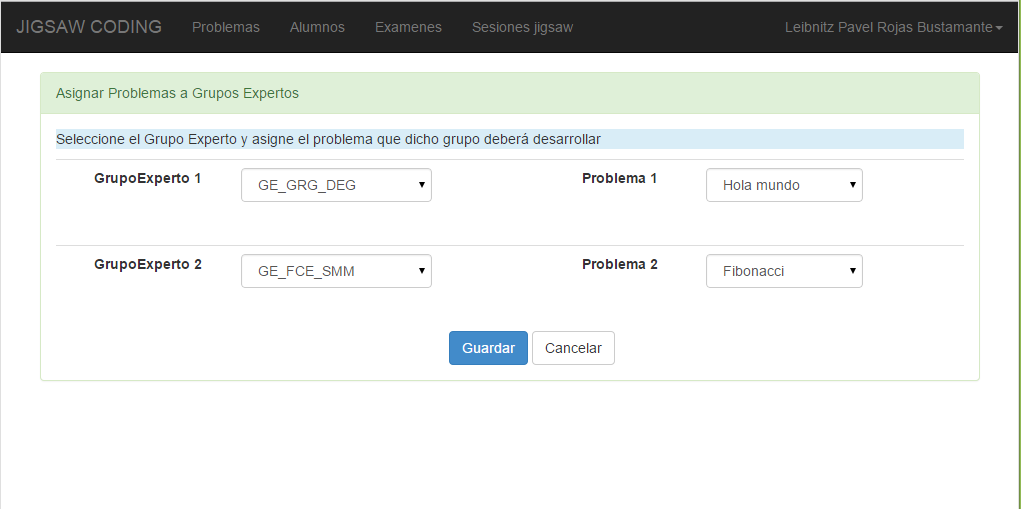
\includegraphics[scale=0.5]{figuras/usodelsistema/docente/sesionesjigsaw_nuevo_07}}
	\end{figure}
	\item Presione el botón Guardar luego de haber asignado a todos los grupos expertos su respectivo problema. El sistema lo redirigirá hacia el panel principal de sesiones jigsaw. \autoref{fig:sesionesjigsaw_nuevo_08}
	\begin{figure}[h!]
		\centering
		\caption{Sistema Jigsaw Coding - Nueva sesión jigsaw}
		\label{fig:sesionesjigsaw_nuevo_08}
		\fbox{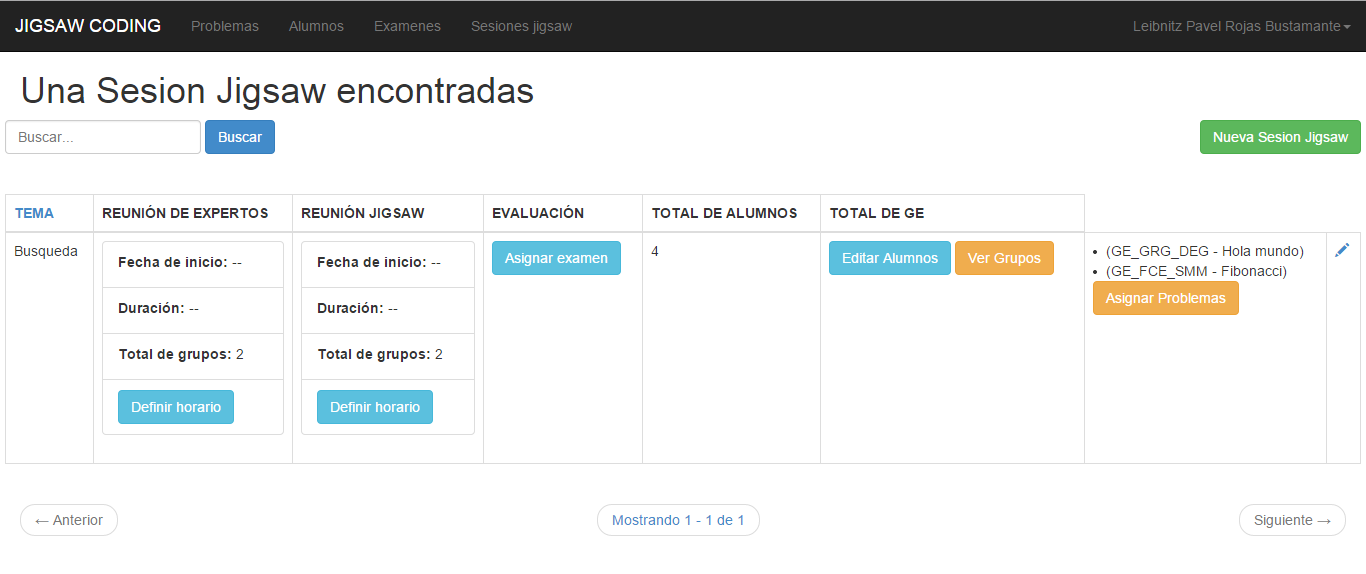
\includegraphics[scale=0.4]{figuras/usodelsistema/docente/sesionesjigsaw_nuevo_08}}
	\end{figure}
	\item Para la fase de evaluación, presione el botón Asignar Examen para seleccionar el examen que será incluído en la sesión jigsaw. \autoref{fig:sesionesjigsaw_nuevo_09}
	\begin{figure}[h!]
		\centering
		\caption{Sistema Jigsaw Coding - Asignar examen a sesión jigsaw}
		\label{fig:sesionesjigsaw_nuevo_09}
		\fbox{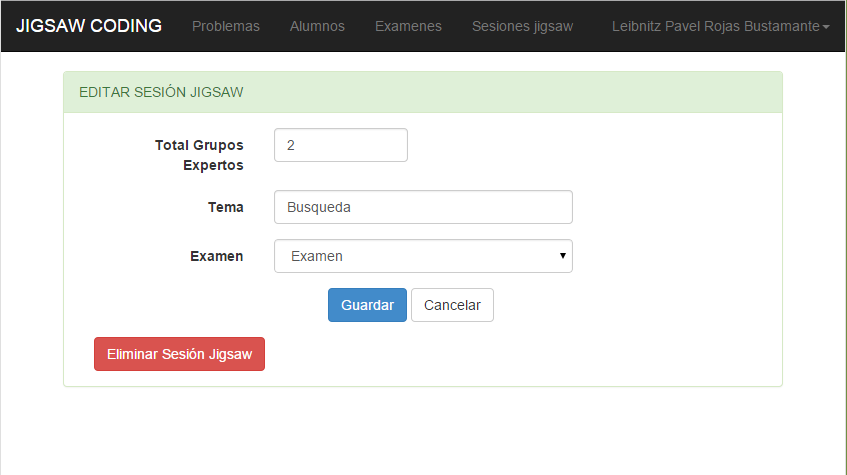
\includegraphics[scale=0.5]{figuras/usodelsistema/docente/sesionesjigsaw_nuevo_09}}
	\end{figure}
	\item Presione el botón Definir Horario para establecer la fecha y hora de inicio para la reunión de expertos, así como también la duración de la misma. \autoref{fig:sesionesjigsaw_nuevo_11}
	\begin{figure}[h!]
		\centering
		\caption{Sistema Jigsaw Coding - Definir horario de reunión de expertos}
		\label{fig:sesionesjigsaw_nuevo_11}
		\fbox{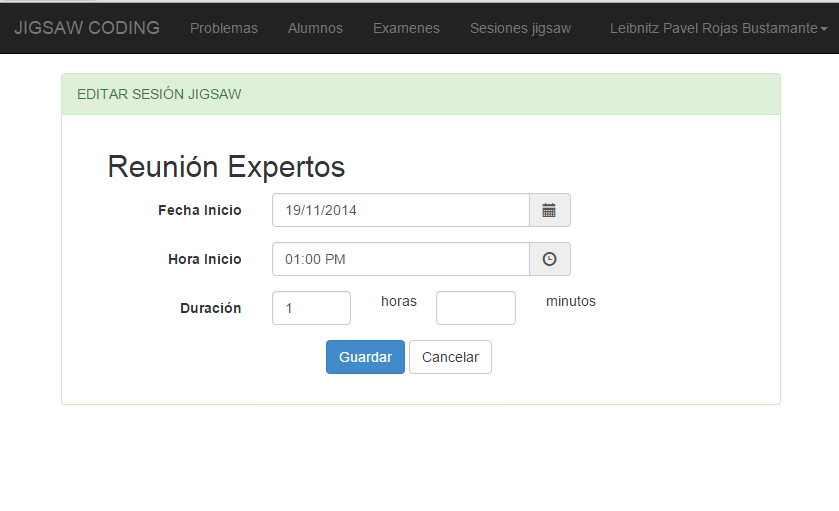
\includegraphics[scale=0.5]{figuras/usodelsistema/docente/sesionesjigsaw_nuevo_11}}
	\end{figure}
	\item Presione el botón Definir Horario para establecer la fecha y hora de inicio para la reunión jigsaw, así como también la duración de la misma. \autoref{fig:sesionesjigsaw_nuevo_13}
	\begin{figure}[h!]
		\centering
		\caption{Sistema Jigsaw Coding - Definir horario de reunión jigsaw}
		\label{fig:sesionesjigsaw_nuevo_13}
		\fbox{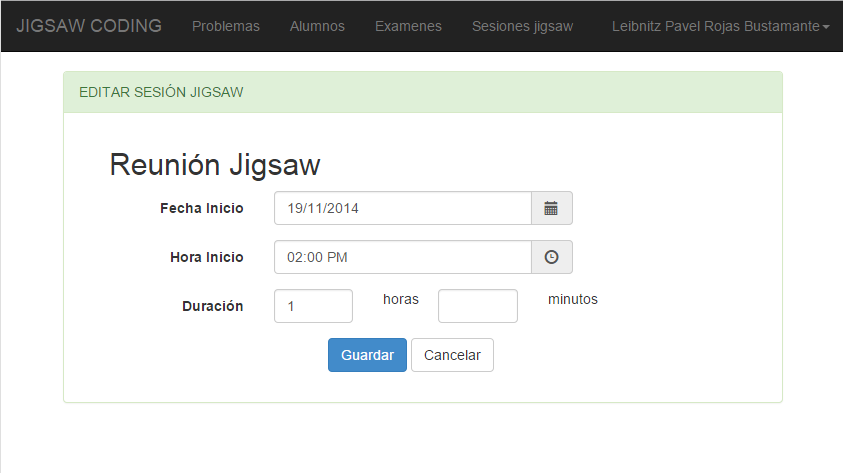
\includegraphics[scale=0.5]{figuras/usodelsistema/docente/sesionesjigsaw_nuevo_13}}
	\end{figure}
	\item Presione el botón Definir Horario para establecere la fecha y hora de inicio para la evaluación, así como también la duración de la misma. \autoref{fig:sesionesjigsaw_nuevo_15}
	\begin{figure}[h!]
		\centering
		\caption{Sistema Jigsaw Coding - Definir horario de examen}
		\label{fig:sesionesjigsaw_nuevo_15}
		\fbox{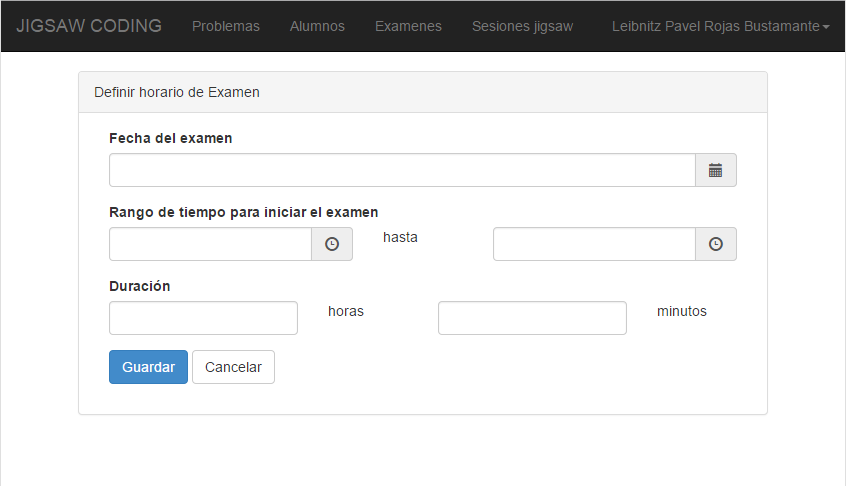
\includegraphics[scale=0.5]{figuras/usodelsistema/docente/sesionesjigsaw_nuevo_15}}
	\end{figure}
\end{enumerate}

\subsection{Unirse a reunión de expertos}
Para que un usuario con perfil Alumno pueda unirse a una reunión de expertos, debe seguir los siguientes pasos:

\begin{enumerate}
	\item Inicie sesión en el Sistema Jigsaw Coding. Si el logueo se realiza exitosamente, entonces, en la pantalla principal del perfil alumno se motrará el listado de sesiones jigsaw a las cuales el alumno puede tener acceso.\autoref{fig:c4_alumno_principal}
	
	\begin{figure}[h!]
		\centering
		\caption{Sistema Jigsaw Coding - Perfil alumno}
		\label{fig:c4_alumno_principal}
		\fbox{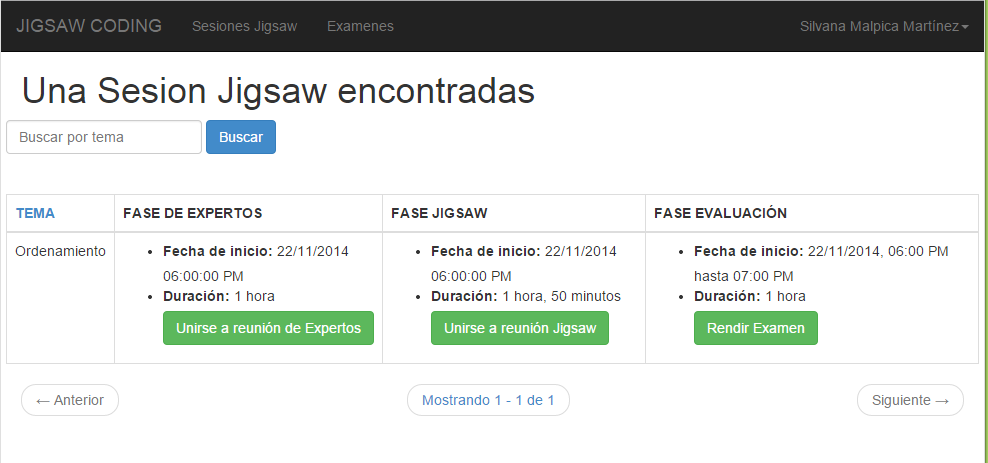
\includegraphics[scale=0.5]{figuras/usodelsistema/alumno/principal}}
	\end{figure}
	
	\item Presione el botón \textbf{Unirse a reunión de Expertos}. A continuación el sistema le mostrará el panel de la reunión de expertos. 
	
	\begin{figure}[h!]
		\centering
		\caption{Sistema Jigsaw Coding - Unirse a reunión de expertos}
		\label{fig:c4_reunion_expertos}
		\fbox{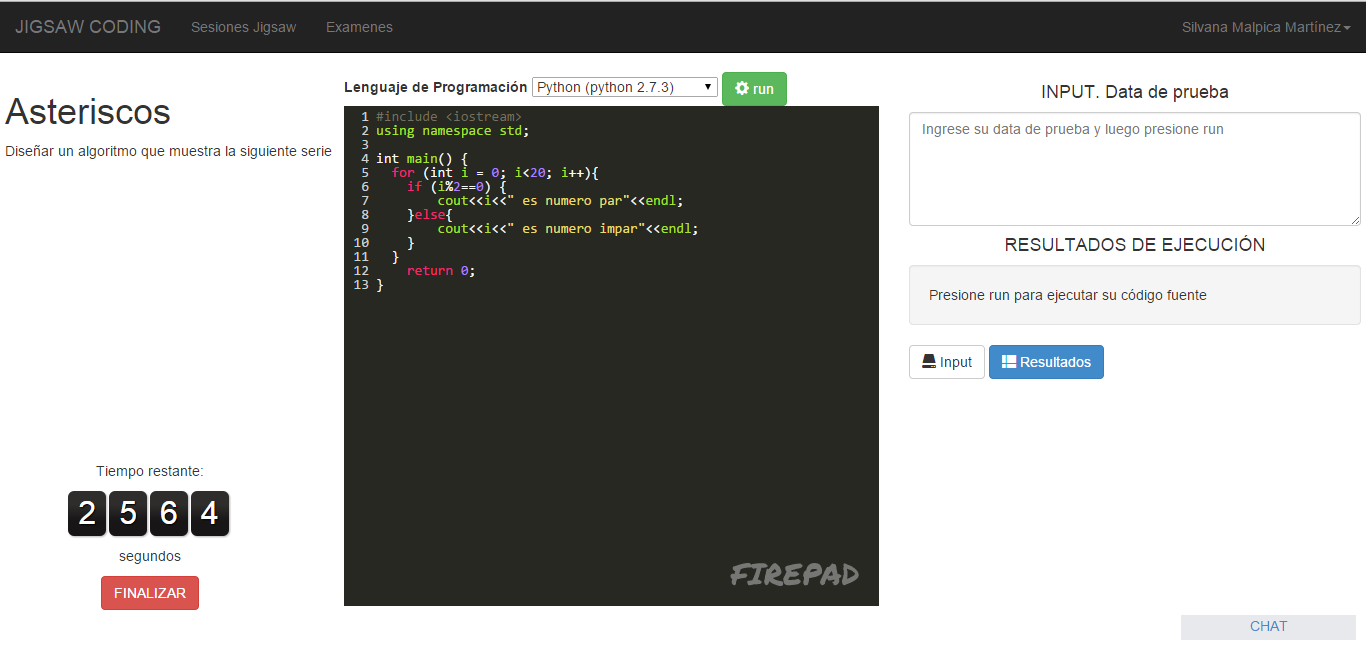
\includegraphics[scale=0.4]{figuras/usodelsistema/alumno/reunion_expertos}}
	\end{figure}
	
	En el panel de reunión de expertos (\autoref{fig:c4_reunion_expertos}) se encontrará lo siguiente: 

	\begin{itemize}
		\item Enunciado del problema.
		\item Editor colaborativo de código fuente.
		\item Menú desplegable para seleccionar el lenguaje de programación(Python, C++ o Java).
		\item Cuadro de texto para ingresar datos de prueba.
		\item Panel de resultados de ejecución.
		\item Chat para comunicarse con el resto de integrantes del grupo experto.
		\item Reloj que marca los segundos restantes para finalizar la reunión de expertos.
	\end{itemize}
\end{enumerate}


\subsection{Unirse a reunión jigsaw}
Para que un usuario con perfil Alumno pueda unirse a una reunión jigsaw, debe seguir los siguientes pasos:

\begin{enumerate}
	\item Inicie sesión en el Sistema Jigsaw Coding. Si el logueo se realiza exitosamente, entonces, en la pantalla principal del perfil alumno se motrará el listado de sesiones jigsaw a las cuales el alumno puede tener acceso.\autoref{fig:c4_alumno_principal}
	\item Presione el botón \textbf{Unirse a reunión Jigsaw}. A continuación el sistema le mostrará el panel de la reunión jigsaw. 
	
	\begin{figure}[h!]
		\centering
		\caption{Sistema Jigsaw Coding - Unirse a reunión jigsaw}
		\label{fig:c4_reunion_jigsaw}
		\fbox{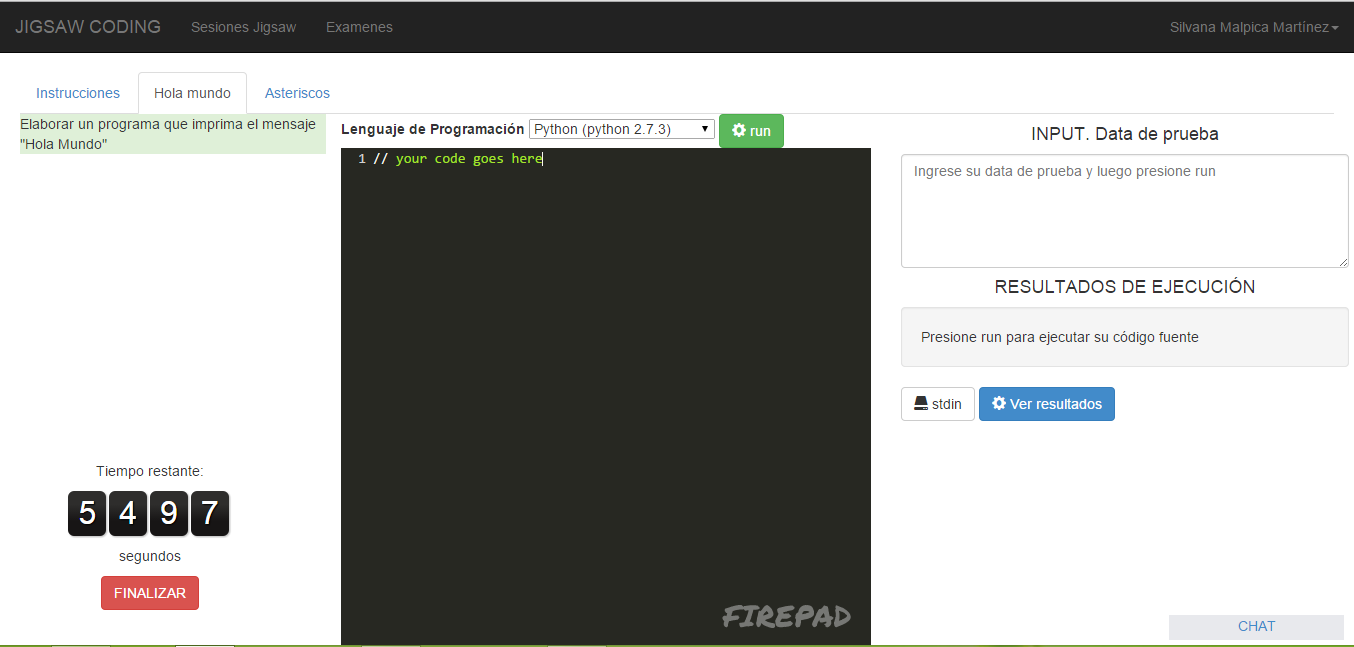
\includegraphics[scale=0.4]{figuras/usodelsistema/alumno/reunion_jigsaw}}
	\end{figure}
	
	En el panel de reunión jigsaw  (\autoref{fig:c4_reunion_jigsaw}) se encontrará lo siguiente: 
	
	\begin{itemize}
		\item Una pestaña con instrucciones que los miembros del grupos jigsaw deben tener en cuenta durante la reunión jigsaw.
		\item Una pestaña por cada problema que el grupo debe resolver.
		\item Enunciado de cada uno de los problemas.
		\item Editor colaborativo de código fuente para cada problema.
		\item Menú desplegable para seleccionar el lenguaje de programación(Python, C++ o Java).
		\item Cuadro de texto para ingresar datos de prueba para cada problema.
		\item Panel de resultados de ejecución para cada problema.
		\item Chat para comunicarse con el resto de integrantes del grupo jigsaw.
		\item Reloj que marca los segundos restantes para finalizar la reunión jigsaw.
	\end{itemize}
\end{enumerate}

\subsection{Rendir evaluación}
Para que un usuario con perfil Alumno pueda rendir un examen, debe seguir los siguientes pasos:

\begin{enumerate}
	\item Inicie sesión en el Sistema Jigsaw Coding. Si el logueo se realiza exitosamente, entonces, en la pantalla principal del perfil alumno se motrará el listado de sesiones jigsaw a las cuales el alumno puede tener acceso.\autoref{fig:c4_alumno_principal}
	\item Presione el botón \textbf{Rendir Examen}. A continuación el sistema le mostrará el panel del examen.
	
	\begin{figure}[h!]
		\centering
		\caption{Sistema Jigsaw Coding - Rendir examen}
		\label{fig:c4_rendir_examen}
		\fbox{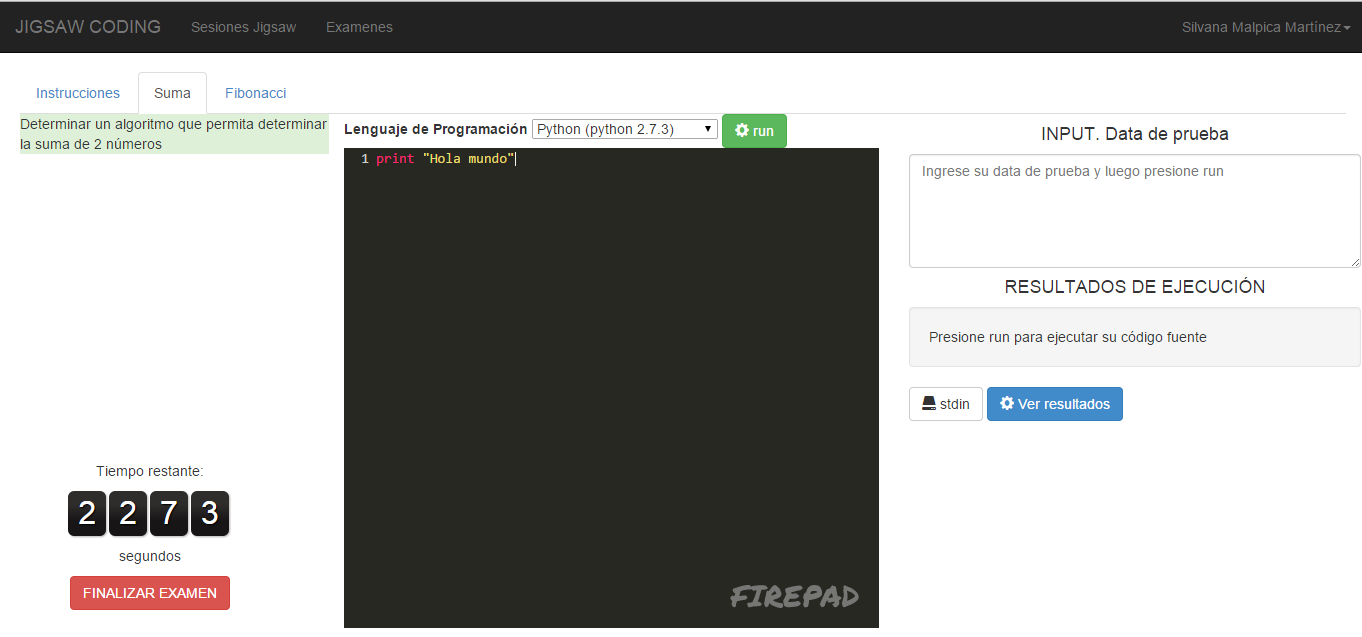
\includegraphics[scale=0.4]{figuras/usodelsistema/alumno/rendir_examen}}
	\end{figure}
	
	En el panel de examen  (\autoref{fig:c4_rendir_examen}) se encontrará lo siguiente: 
	
	\begin{itemize}
		\item Una pestaña con instrucciones que el alumno deben tener en cuenta durante el examen.
		\item Una pestaña por cada problema que el alumno debe resolver.
		\item Enunciado de cada uno de los problemas.
		\item Editor de código fuente para cada problema.
		\item Menú desplegable para seleccionar el lenguaje de programación(Python, C++ o Java).
		\item Cuadro de texto para ingresar datos de prueba para cada problema.
		\item Panel de resultados de ejecución para cada problema.
		\item Reloj que marca los segundos restantes para finalizar el examen.
	\end{itemize}
	
	\item Luego de rendir el examen, el alumno debe esperar a que el docente califique sus respuestas y le asigne una nota, la cual podrá ser vista en el menú \textbf{Examenes}. \autoref{fig:c4_nota_de_examen}
	
	\begin{figure}[h!]
		\centering
		\caption{Sistema Jigsaw Coding - Ver nota de examen}
		\label{fig:c4_nota_de_examen}
		\fbox{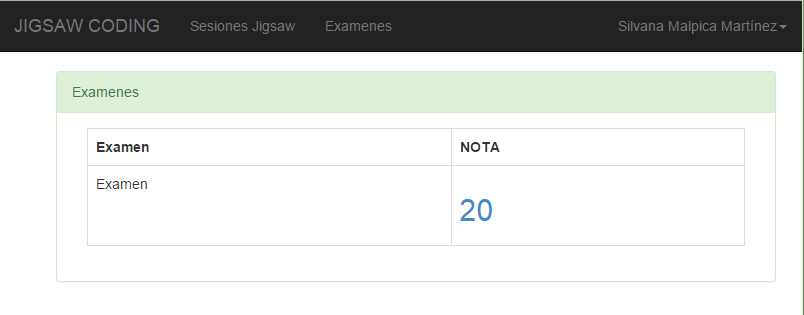
\includegraphics[scale=0.4]{figuras/usodelsistema/alumno/nota_de_examen}}
	\end{figure}
	
\end{enumerate}
\clearpage
\section{Definición de métricas de calidad para el Sistema Jigsaw Coding}
\label{sec:metricas_calidad}
A continuación se presentan las métricas de calidad que se van a medir en Sistema Jigsaw Coding. Estas métricas están basadas en la norma ISO-9126, la cual establece un estándar internacional para la evaluación de la calidad de los productos software \cite{iso9126-3}.

\subsection{Entendibilidad}
La presente métrica se refiere a la característica de \textit{Usabilidad} , donde se medirá el grado de \textit{Entendibilidad} que tiene el Sistema para los usuarios. \autoref{tab:c4_entendibilidad}
\begin{longtable}{L{4cm}L{8cm}}
	\caption{Métrica de calidad: Entendibilidad}
	\label{tab:c4_entendibilidad}\\
	\toprule[0.8mm]
	\textbf{Nombre de la métrica} & \textbf{Entendibilidad del Sistema Jigsaw Coding}\\
	\midrule
	Código & MC-\metrica\\
	\midrule
	Característica & Usabilidad \\
	\midrule
	Sub-característica & Entendibilidad\\
	\midrule
	Propósito & ¿Qué porcentaje de los usuarios consideran que las funcionalidades del sistema son fáciles o muy fáciles de entender? \\
	\midrule
	Método de aplicación & Realizar una encuesta:
	¿Qué tan fácil o difícil le resultó entender las funcionalidades del sistema?
	\begin{itemize}
		\item Muy fácil
		\item Fácil
		\item Ni fácil ni difícil
		\item Difícil
		\item Muy difícil
	\end{itemize}\\
	\midrule
	\multirow{3}{*}{ \parbox{4cm}{ Medición, fórmula y elementos medibles}   } & $$x = \frac{A}{B} $$\\
	& A : Cantidad de usuarios que selecionaron la alternativa Fácil o Muy fácil.\\
	& B : Cantidad de usuarios encuestados.	\\
	\midrule
	Tipo de medida & A,B: contador \\
	\midrule
	Interpretación del valor & Lo más cercano a 1 es mejor \\
	\midrule
	Tipo de escala & Absoluta \\
	\bottomrule[0.8mm]	
\end{longtable}




%\subsection{Adecuación}
%Esta métrica se refiere a la característica de \textit{Funcionalidad} , donde se medirá el nivel de \textit{Adecuación} que tiene el Sistema Jigsaw Coding. \autoref{tab:c4_adecuacion}
%\begin{longtable}{L{4cm}L{8cm}}
%	\caption{Métrica de calidad: Adecuación}
%	\label{tab:c4_adecuacion}\\
%	\toprule[0.8mm]
%	\textbf{Nombre de la métrica} & \textbf{Adecuación del Sistema Jigsaw Coding}\\
%	\midrule
%	Código & MC-\metrica\\
%	\midrule
%	Característica &  Funcionalidad\\
%	\midrule
%	Sub-característica & Adecuación\\
%	\midrule
%	Propósito &  ¿Qué cantidad de casos de uso no se encuentran dentro de las funcionalidades del sistema jigsaw coding?\\
%	\midrule
%	Método de aplicación & Contar el total de casos de uso que no se pueden realizar a través del sistema jigsaw coding\\
%	\midrule
%	\multirow{3}{*}{ \parbox{4cm}{ Medición, fórmula y elementos medibles}   } & $$x = \frac{A}{B} $$\\
%	& A : Cantidad de casos de uso implementados en el sistema.\\
%	& B : Cantidad de casos de uso especificados en el \autoref{apendice.A}	\\
%	\midrule
%	Tipo de medida & A,B: Contador \\
%	\midrule
%	Interpretación del valor &  Lo más cercano a 1 es mejor\\
%	\midrule
%	Tipo de escala & Absoluta \\
%	\bottomrule[0.8mm]
%\end{longtable}

\subsection{Portabilidad}
La presente métrica se refiere a la característica de \textit{Portabilidad} , en la que se medirá el grado de \textit{Adaptabilidad} que tiene el Sistema desarrollado. \autoref{tab:c4_portabilidad}
\begin{longtable}{L{4cm}L{8cm}}
	\caption{Métrica de calidad: Portabilidad}
	\label{tab:c4_portabilidad}\\
	\toprule[0.8mm]
	\textbf{Nombre de la métrica} & \textbf{Portabilidad del Sistema Jigsaw Coding}\\
	\midrule
	Código & MC-\metrica\\
	\midrule
	Característica & Portabilidad \\
	\midrule
	Sub-característica & Adaptabilidad\\
	\midrule
	Propósito &  ¿En cuántos navegadores web puede usarse el sistema sin tener problemas?\\
	\midrule
	Método de aplicación & Utilizar el sistema en diversos navegarores y contar en cuántos de ellos el sistema funciona correctamente.\\
	\midrule
	\multirow{2}{*}{ \parbox{4cm}{ Medición, fórmula y elementos medibles}   } & $$x = n $$\\
	& n : Número de navegadores web en los que el sistema funciona correctamente.\\
	\midrule
	Tipo de medida &  n: Contador\\
	\midrule
	Interpretación del valor &  A mayor valor de $x$ mejor.\\
	\midrule
	Tipo de escala &  Absoluta\\
	\bottomrule[0.8mm]
\end{longtable}


\subsection{Eficiencia}
La presente métrica se refiere a la característica de \textit{Eficiencia} , donde se medirá el \textit{Tiempo de respuesta} que tiene el Sistema. \autoref{tab:c4_eficiencia}.
\begin{longtable}{L{4cm}L{8cm}}
	\caption{Métrica de calidad: Eficiencia}
	\label{tab:c4_eficiencia}\\
	\toprule[0.8mm]
	\textbf{Nombre de la métrica} & \textbf{Eficiencia del Sistema Jigsaw Coding}\\
	\midrule
	Código & MC-\metrica\\
	\midrule
	Característica & Eficiencia \\
	\midrule
	Sub-característica & Tiempo de respuesta\\
	\midrule
	Propósito & ¿Cuál es el promedio de tiempo de respuesta del Sistema Jigsaw Coding? \\
	\midrule
	Método de aplicación & Medir el tiempo de respuesta de las funcionalidades más importantes del sistema: Generar grupos, Unirse a Reunión de Expertos, Unirse a Reunión Jigsaw, Rendir Examen, Resolver problema(Compilar).\\
	\midrule
	\multirow{2}{*}{ \parbox{4cm}{ Medición, fórmula y elementos medibles}   } 
	& $$x = \sum_{i}^{n}{t_{i}} $$\\
	& $t_{i}$ : Tiempo de respuesta en milisegundos de la funcionalidad $i$.\\
	\midrule
	Tipo de medida & $t_{i}$: milisegundos \\
	\midrule
	Interpretación del valor & Lo más cercano a 0 es mejor \\
	\midrule
	Tipo de escala & Absoluta \\
	\bottomrule[0.8mm]	
\end{longtable}

%\begin{longtable}{L{4cm}L{8cm}}
%	\toprule[0.8mm]
%	\textbf{Nombre de la métrica} & \textbf{}\\
%	\midrule
%	Código & MC-\metrica\\
%	\midrule
%	Característica &  \\
%	\midrule
%	Sub-característica & \\
%	\midrule
%	Propósito &  \\
%	\midrule
%	Método de aplicación &\\
%	\midrule
%	Medición, fórmula y elementos medibles
%	& 	\\
%	\midrule
%	Tipo de medida &  \\
%	\midrule
%	Interpretación del valor &  \\
%	\midrule
%	Tipo de escala &  \\
%	\bottomrule[0.8mm]
%\end{longtable}









































